%!TEX root = ../main.tex

\chapter{Application of the Model}\label{cha:applying-model}

In this Chapter a method for assessing the sensitivity of the model will be outlined.
This is done by making several small changes to the parameters of strategies and observing whether the model can discriminate between the new altered vectors.
The size of the change made to the strategy will be varied and the models performance recorded for each deviation.
It is expected that there is a cut-off where the model changes from performing well to performing badly, and this gives an approximation of it's sensitivity.
Finally, model will be applied to the Axelrod-Python library to determine if it contains any duplicate strategies.



\section{MemoryOne Strategies}

A MemoryOne strategy bases its decision entirely on the the last round of play.
In Axelrod-Python they are defined by a vector $v$ of length 4 that determines the probability of Cooperation given the previous rounds history, ie:
$$
v = (P(C|CC), P(C|CD), P(C|DC), P(C|DD))
$$
For example, a MemoryOne strategy defined by the vector $v=(1, 1, 1, 1)$ is equivalent to Cooperator.
TitForTat can be implemented as a MemoryOne player with the vector $v=(1, 0, 1, 0)$, Pavlov as the MemoryOne player with $v=(1, 0, 0, 1)$ and Random as the MemoryOne player with $v=(0.5, 0.5, 0.5, 0.5)$.
See Section \ref{sec:individual_strategies} for explanations of how these strategies operate.



\section{Determining the sensitivity of the Model}

All possible MemoryOne strategies are defined by the space $S = [0, 1]^4_{\mathbb{R}}$.
For a vector $s \in S$ and a deviation $\delta \in (0, 1)$, 16 new deviated vectors are created by taking the sum of $s$ with all possible vectors $(\pm \delta, \pm \delta, \pm \delta, \pm \delta)$, but bounding each element in the range $[0, 1]$.
For example, with $s = (0.2, 0, 0.5, 0.95)$ and $\delta = 0.1$, the 16 vectors produced are:

\begin{itemize}
\begin{multicols}{4}
  \item $(0.3, 0.1, 0.6, 1.0)$
  \item $(0.3, 0.1, 0.6, 0.85)$
  \item $(0.3, 0.1, 0.4, 1.0)$
  \item $(0.3, 0.1, 0.4, 0.85)$
  \item $(0.3, 0.0, 0.6, 1.0)$
  \item $(0.3, 0.0, 0.6, 0.85)$
  \item $(0.3, 0.0, 0.4, 1.0)$
  \item $(0.3, 0.0, 0.4, 0.85)$
  \item $(0.1, 0.1, 0.6, 1.0)$
  \item $(0.1, 0.1, 0.6, 0.85)$
  \item $(0.1, 0.1, 0.4, 1.0)$
  \item $(0.1, 0.1, 0.4, 0.85)$
  \item $(0.1, 0.0, 0.6, 1.0)$
  \item $(0.1, 0.0, 0.6, 0.85)$
  \item $(0.1, 0.0, 0.4, 1.0)$
  \item $(0.1, 0.0, 0.4, 0.85)$
\end{multicols}
\end{itemize}

The 16 deviated vectors are then entered into an Ashlock tournament to produce the corresponding results table where all strategies are compared (as described in Section \ref{sec:ashlock_tourn}).
The model is then be applied to this set of results, and the proportion of comparisons predicted correctly is recorded.
As all the strategies have been defined by unique vectors, it is known that all the strategies are different and so the model should predict that they all different.
By repeating this process for different vectors $s \in S$ whilst also varying $\delta$, Figure \ref{fig:m1_correct} is produced.

\begin{figure}[htbp!]
    \centering
    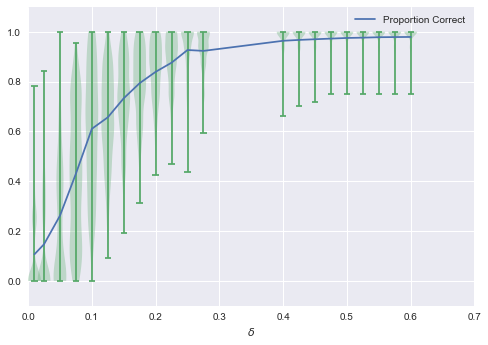
\includegraphics[width=\textwidth]{../img/ML/proportion-correct.png}
    \caption{Caption here}
    \label{fig:m1_correct}
\end{figure}



\section{Applying Model to Axelrod-Python}

The final section of this report addresses the problem of determining when strategies in Axelrod-Python are identical.
The assumption made in Section \ref{sec:training_model} must now be ignored.
It stated: \textit{Strategies with different names are assumed to be different}, but this is not necessarily the case.

In order to determine whether any strategies in Axelrod-Python were identical, all of them were entered into an Ashlock Tournament.
The corresponding results table where all strategies are compared (as described in Section \ref{sec:ashlock_tourn}) was then computed, and the model was applied to this.
A new table could then be produced containing pairs of strategies that the model predicted were equivalent.

In Figure \ref{fig:matrix_similarity}, this table is presented as a Matrix Plot.
Note that the leading diagonal represents strategies being equivalent to themselves, also the plot is symmetric, because if strategy $A$ is similar to strategy $B$ then strategy $B$ is similar to strategy $A$.

\begin{figure}[htbp!]
    \centering
    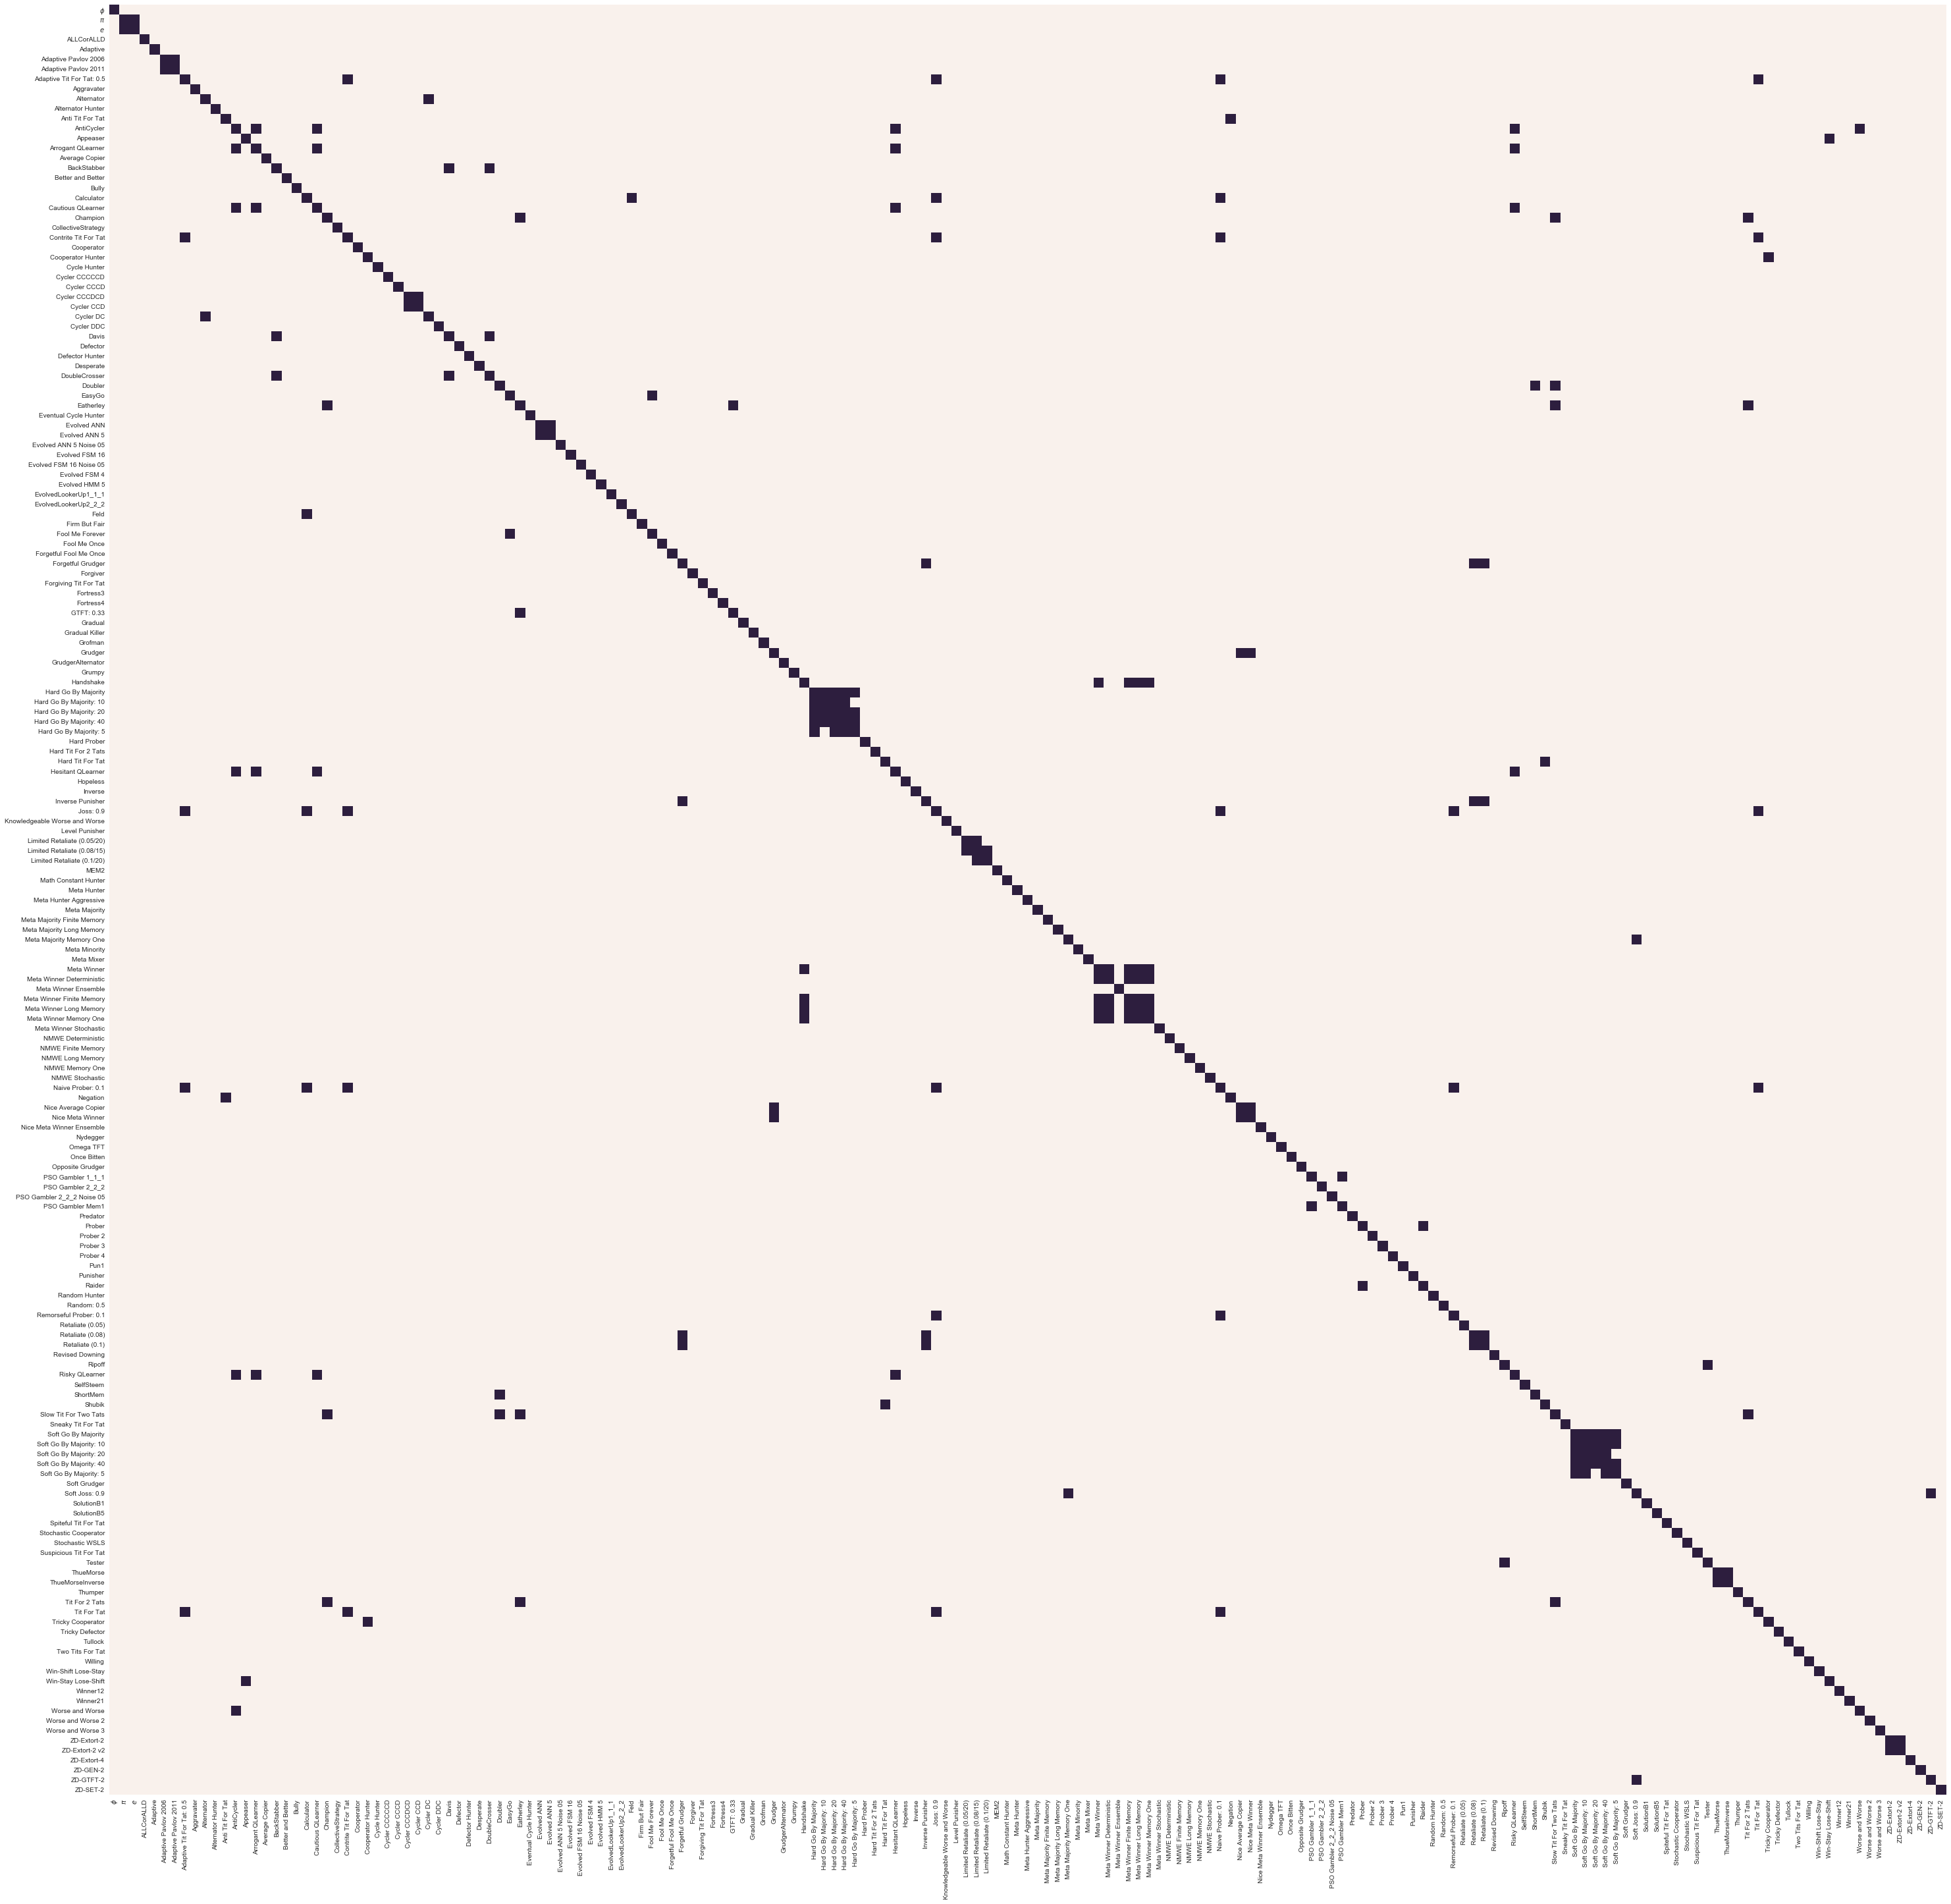
\includegraphics[width=0.8\linewidth]{../img/ML/similarity_heatmap.png}
    \caption{Matrix Plot of similarity}
    \label{fig:matrix_similarity}
\end{figure}

However this plot does not provide much insight.
Instead it can be presented as Network Graph, as in Figure \ref{fig:overall_neighbourhoods}.
Here nodes represent strategies, and edges link nodes that the model predicted to be equivalent.
The graph is undirected for the same reason that Figure \ref{fig:matrix_similarity} is symmetric.
For clarity, strategies that are only similar to themselves have been omitted.

\begin{figure}[htbp!]
    \centering
    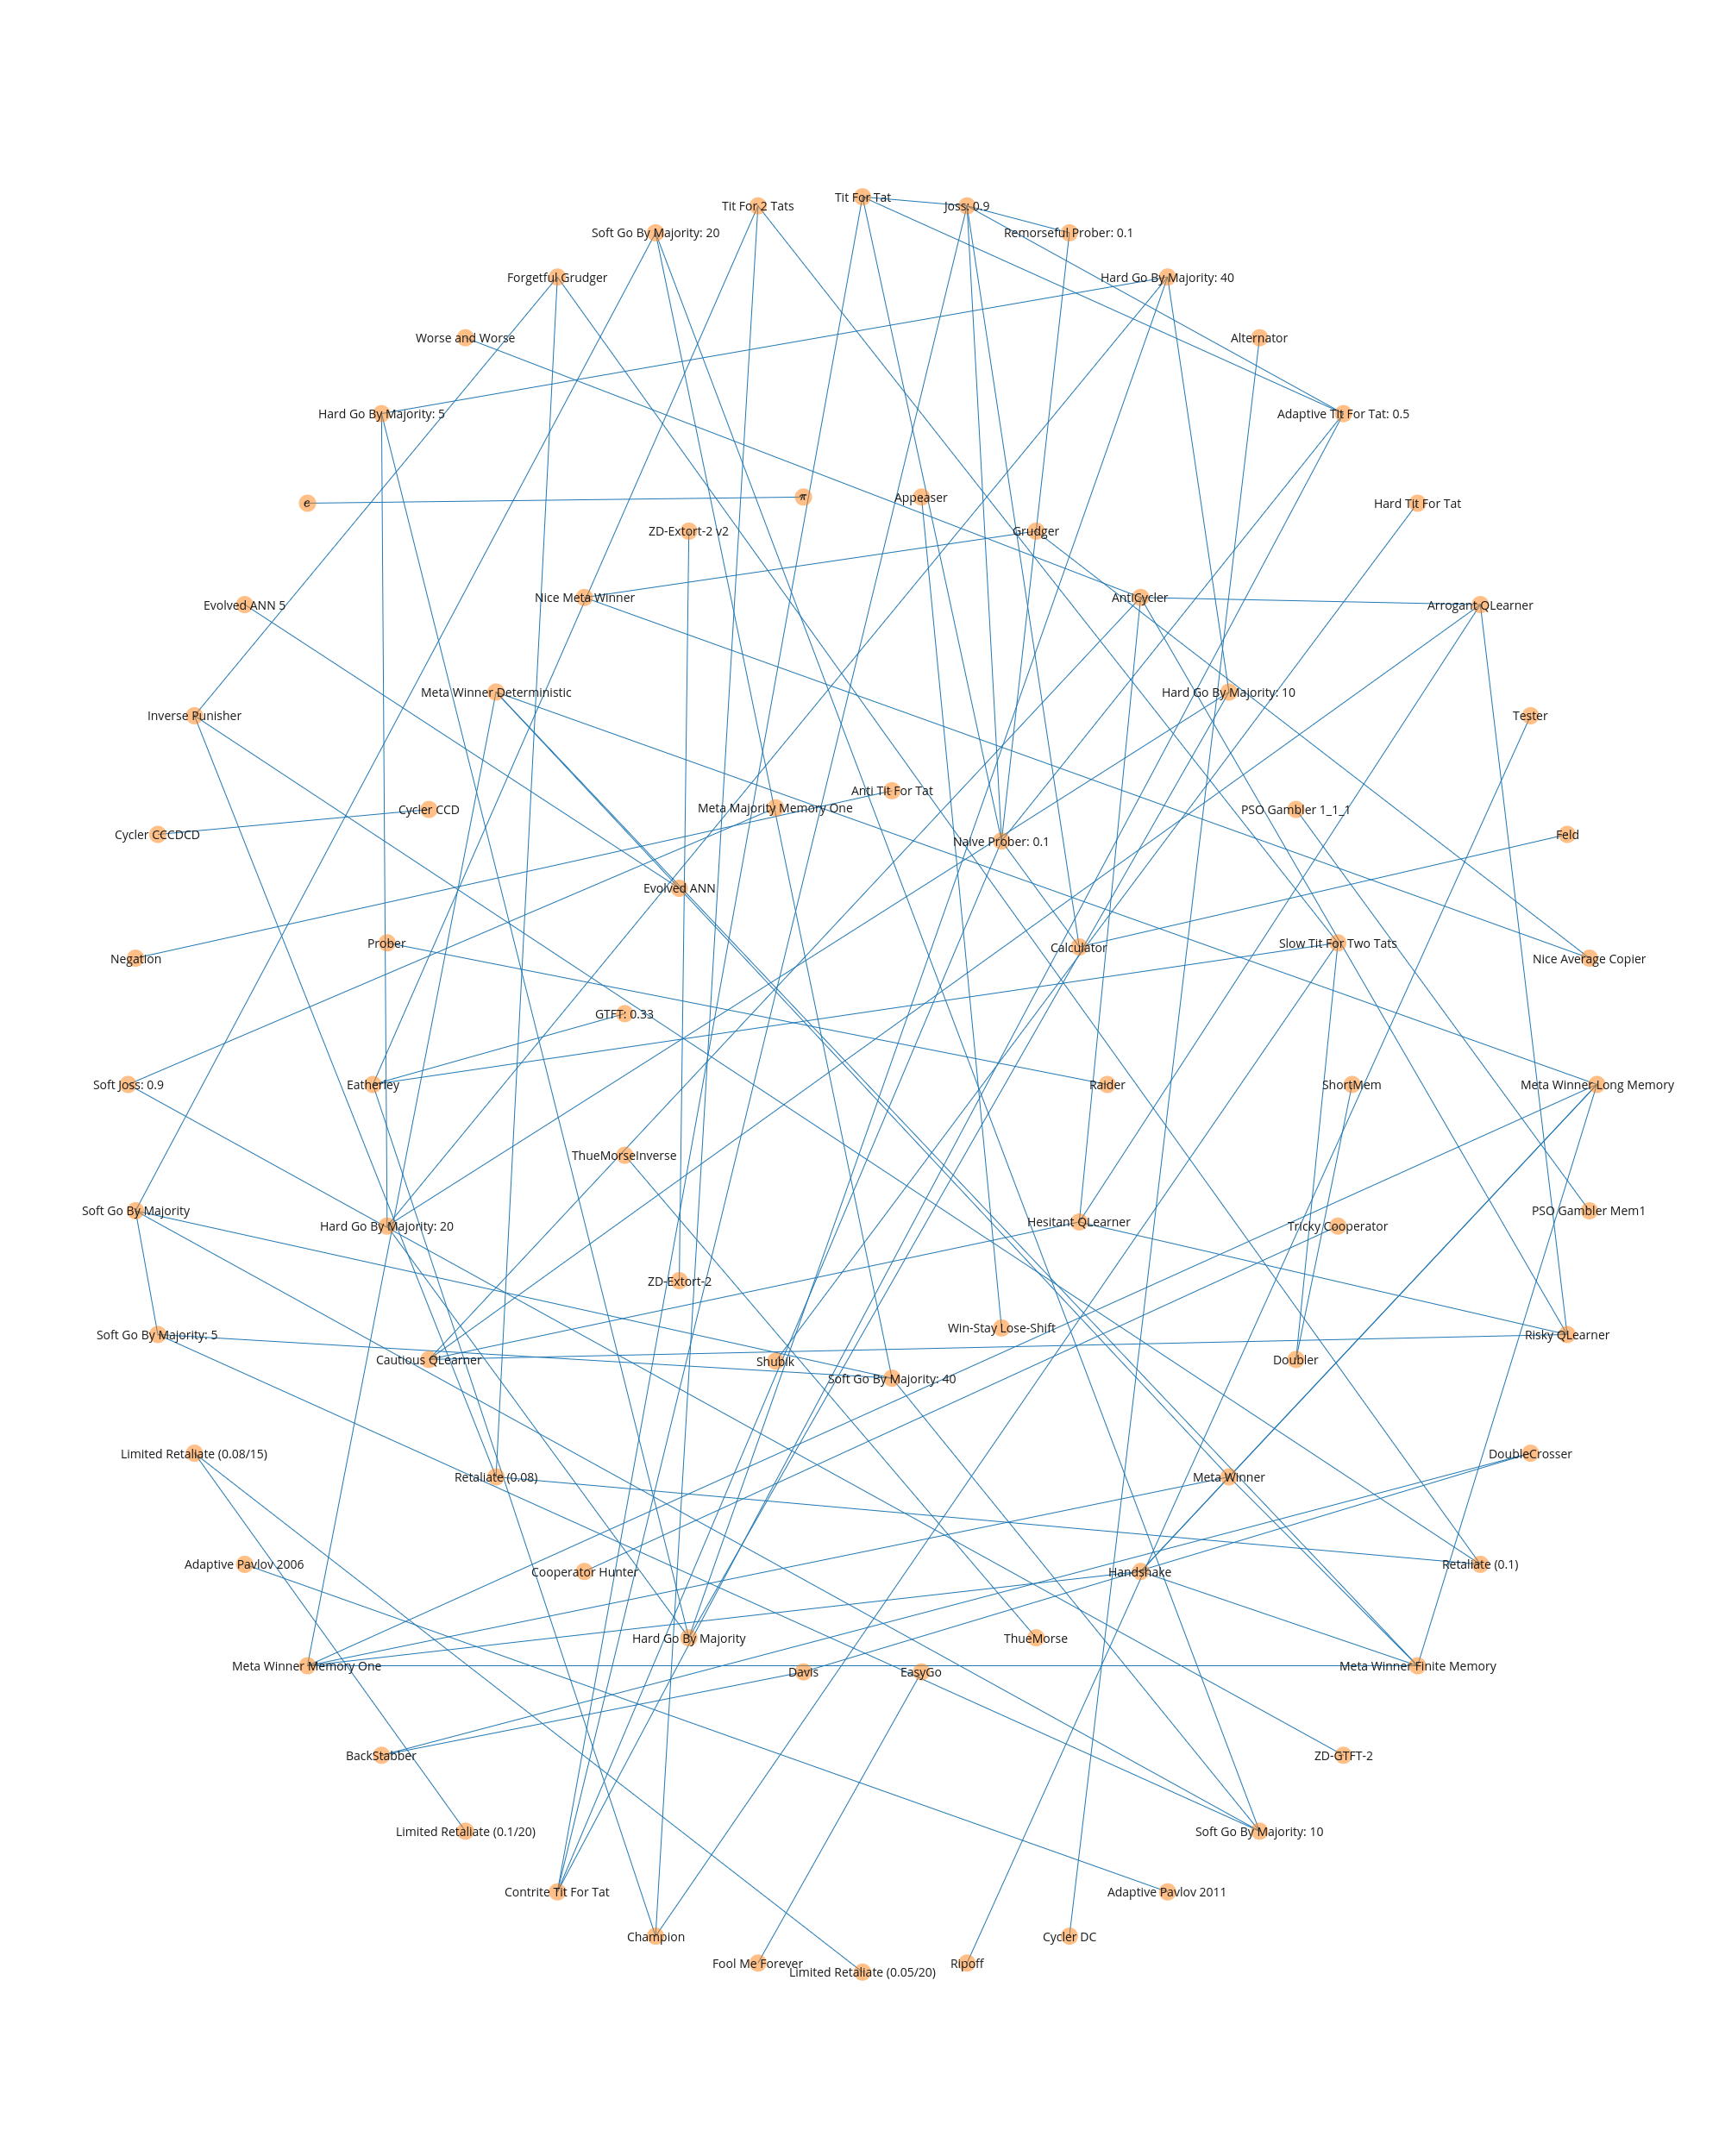
\includegraphics[width=0.8\linewidth]{../img/neighbourhoods/overall.png}
    \caption{Network Graph of strategies that the model had deemed equivalent}
    \label{fig:overall_neighbourhoods}
\end{figure}

In Figure \ref{fig:sep_neighbourhoods}, all of the disjoint neighbourhoods from Figure \ref{fig:overall_neighbourhoods} have been separated out and some of these will now be explored.
Figures \ref{fig:nbh_soft_gbm} and \ref{fig:nbh_hard_gbm} are perfect examples of the model exactly as expected.
Figure \ref{fig:nbh_soft_gbm} shows that the model predicted several SoftGoByMajority strategies to be equivalent to each other.
The only difference between them was the memory depth.
Again in Figure \ref{fig:nbh_hard_gbm} the only difference between the various HardGoByMajority strategies was the memory depth.
However, the model was able to distinguish between all Hard and Soft version of GoByMajority, hence the two networks are disjoint.

In Figure \ref{fig:nbh_alt_cd}


\begin{figure}[htbp!]
\subfloat[]{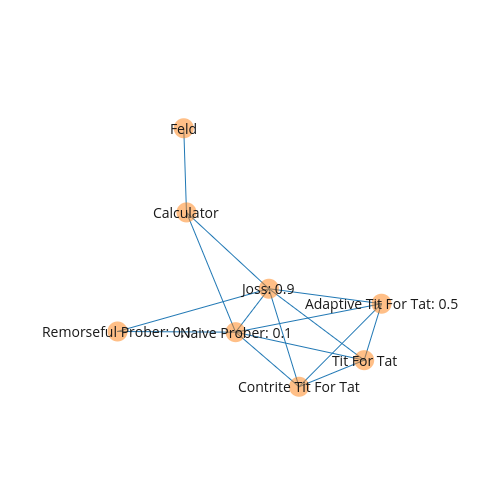
\includegraphics[width = 0.3\textwidth]{../img/neighbourhoods/1.png}}
\subfloat[]{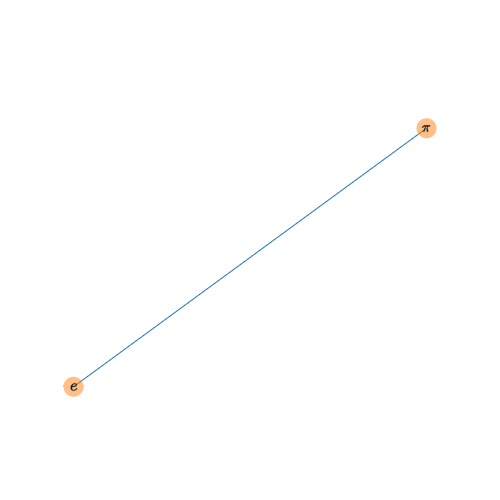
\includegraphics[width = 0.3\textwidth]{../img/neighbourhoods/10.png}\label{fig:nbh_soft_gbm}}
\subfloat[]{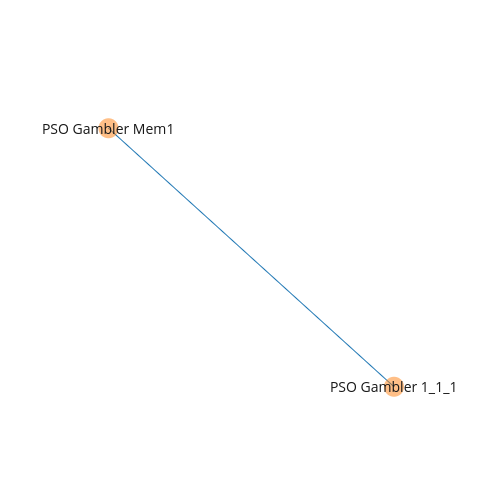
\includegraphics[width = 0.3\textwidth]{../img/neighbourhoods/102.png}} \\
\phantomcaption
\end{figure}
\begin{figure}[htbp!]
\ContinuedFloat
\subfloat[]{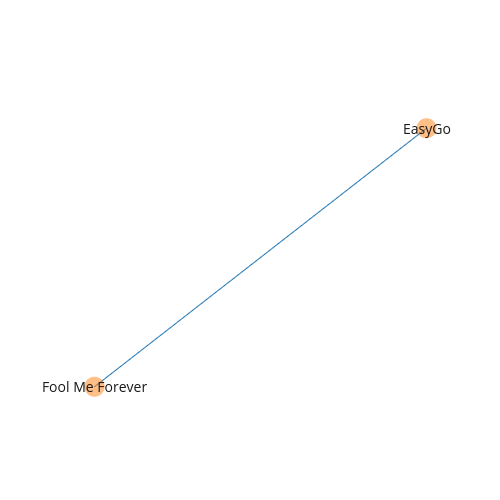
\includegraphics[width = 0.3\textwidth]{../img/neighbourhoods/107.png}}
\subfloat[]{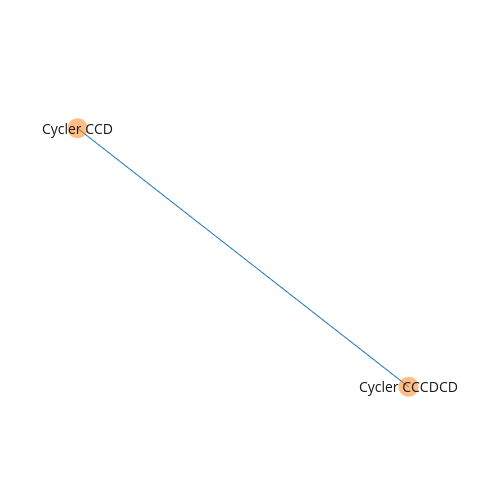
\includegraphics[width = 0.3\textwidth]{../img/neighbourhoods/12.png}}
\subfloat[]{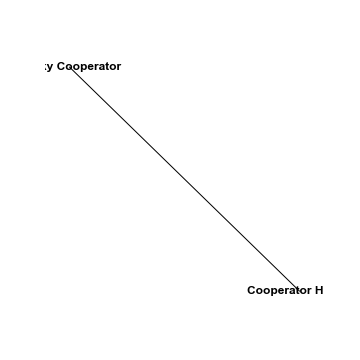
\includegraphics[width = 0.3\textwidth]{../img/neighbourhoods/16.png}} \\
\phantomcaption
\end{figure}
\begin{figure}[htbp!]
\ContinuedFloat
\subfloat[]{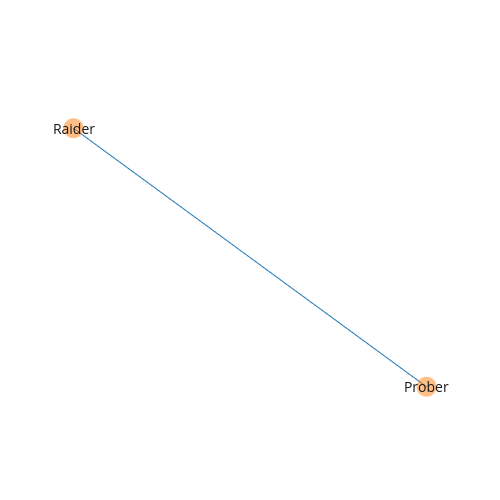
\includegraphics[width = 0.3\textwidth]{../img/neighbourhoods/17.png}}
\subfloat[]{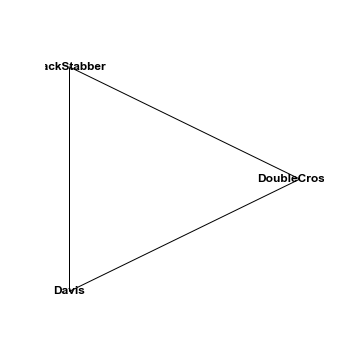
\includegraphics[width = 0.3\textwidth]{../img/neighbourhoods/18.png}}
\subfloat[]{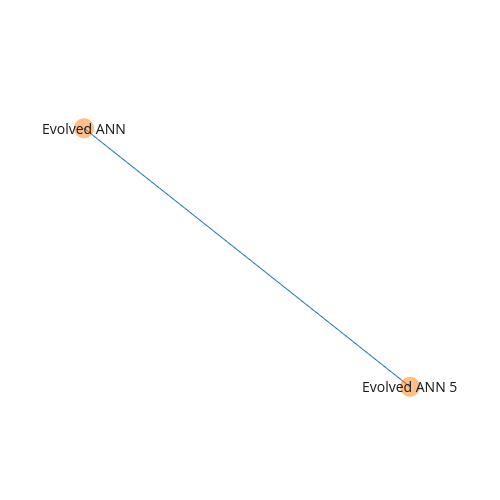
\includegraphics[width = 0.3\textwidth]{../img/neighbourhoods/2.png}} \\
\phantomcaption
\end{figure}
\begin{figure}[htbp!]
\ContinuedFloat
\subfloat[]{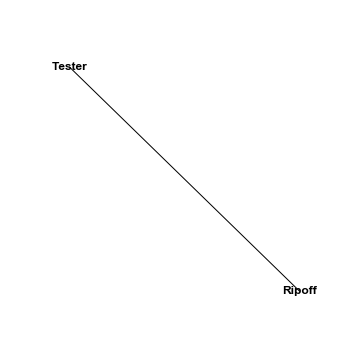
\includegraphics[width = 0.3\textwidth]{../img/neighbourhoods/22.png}}
\subfloat[]{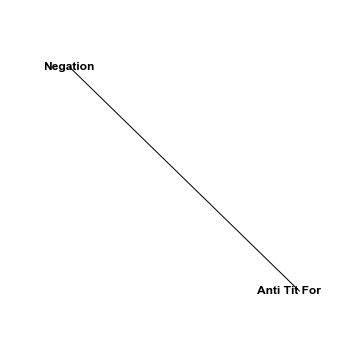
\includegraphics[width = 0.3\textwidth]{../img/neighbourhoods/24.png}}
\subfloat[]{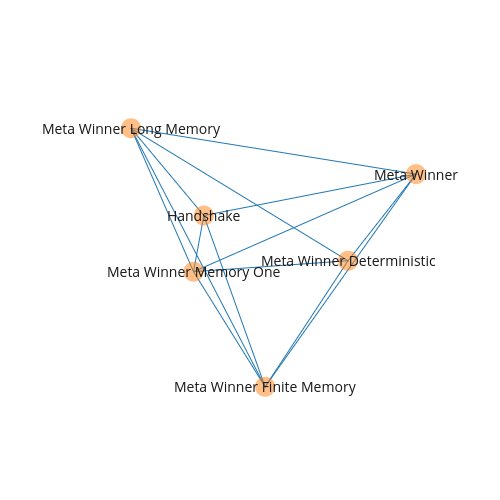
\includegraphics[width = 0.3\textwidth]{../img/neighbourhoods/29.png}} \\
\phantomcaption
\end{figure}
\begin{figure}[htbp!]
\ContinuedFloat
\subfloat[]{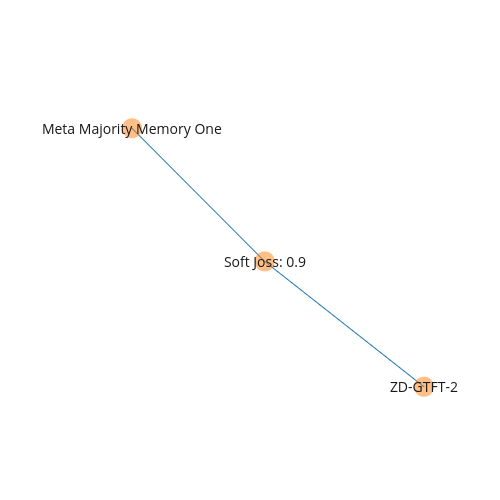
\includegraphics[width = 0.3\textwidth]{../img/neighbourhoods/30.png}}
\subfloat[]{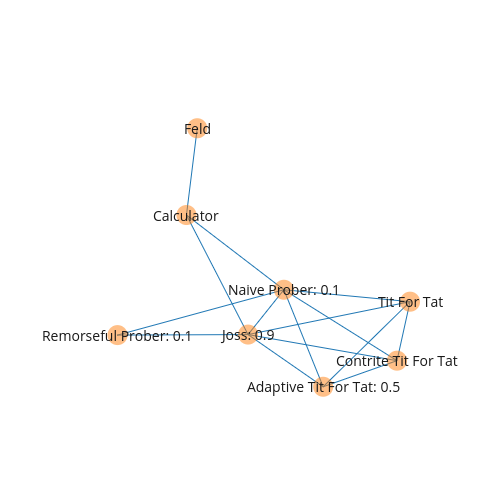
\includegraphics[width = 0.3\textwidth]{../img/neighbourhoods/31.png}}
\subfloat[]{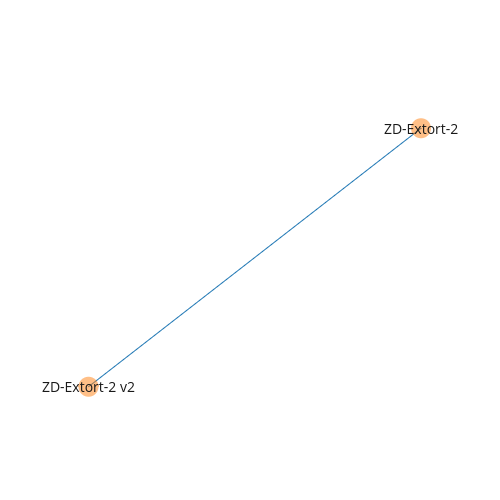
\includegraphics[width = 0.3\textwidth]{../img/neighbourhoods/36.png}} \\
\phantomcaption
\end{figure}
\begin{figure}[htbp!]
\ContinuedFloat
\subfloat[]{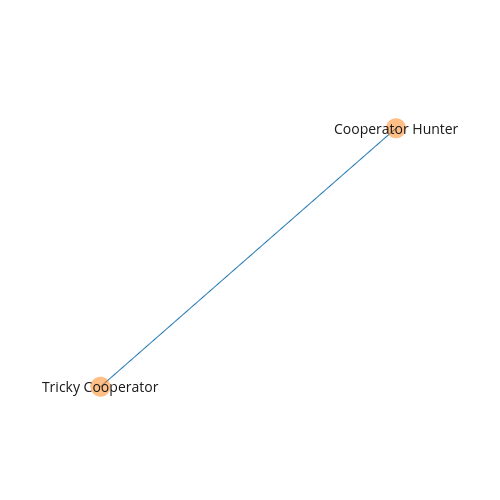
\includegraphics[width = 0.3\textwidth]{../img/neighbourhoods/38.png}}
\subfloat[]{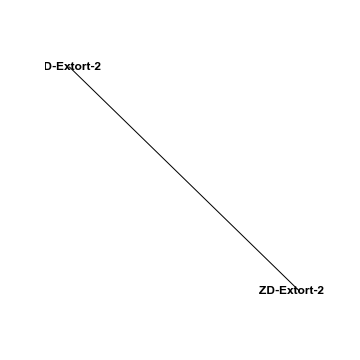
\includegraphics[width = 0.3\textwidth]{../img/neighbourhoods/4.png}}
\subfloat[]{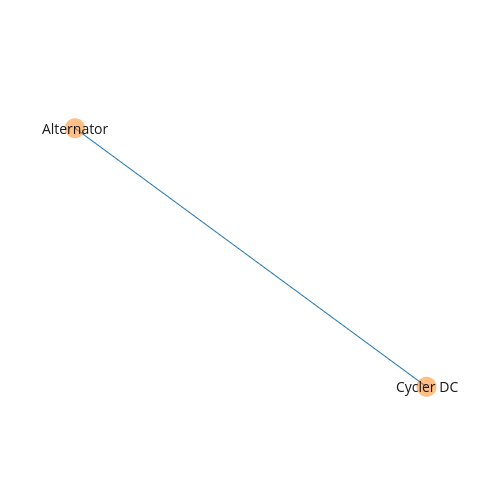
\includegraphics[width = 0.3\textwidth]{../img/neighbourhoods/47.png}\label{fig:nbh_alt_cd}} \\
\phantomcaption
\end{figure}
\begin{figure}[htbp!]
\ContinuedFloat
\subfloat[]{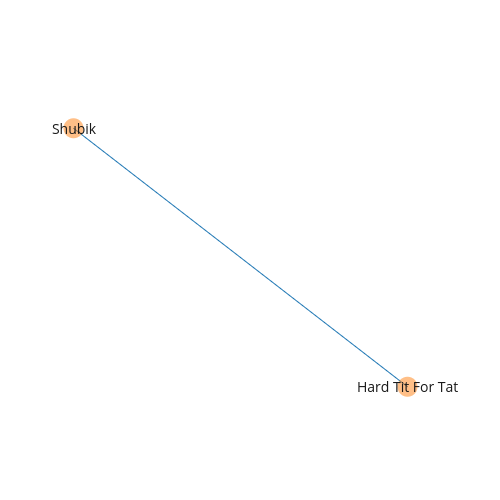
\includegraphics[width = 0.3\textwidth]{../img/neighbourhoods/49.png}}
\subfloat[]{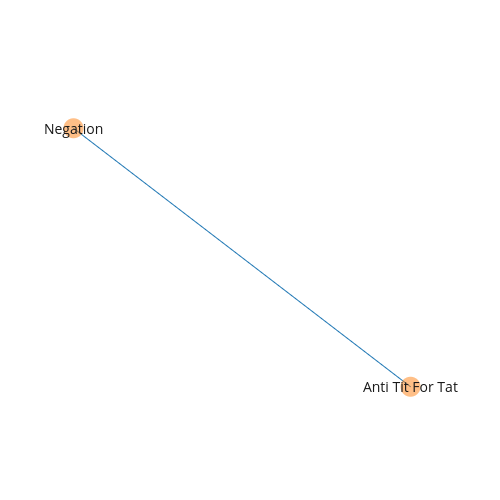
\includegraphics[width = 0.3\textwidth]{../img/neighbourhoods/55.png}}
\subfloat[]{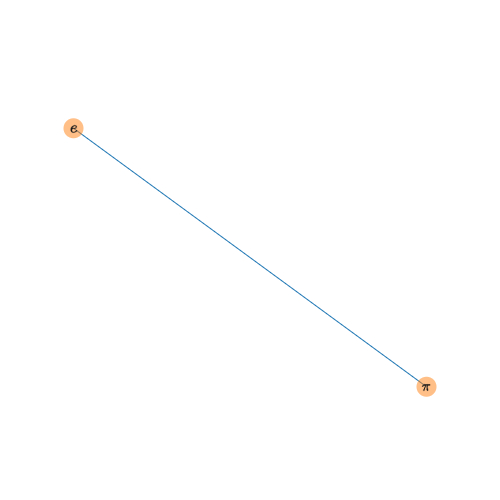
\includegraphics[width = 0.3\textwidth]{../img/neighbourhoods/58.png}} \\
\phantomcaption
\end{figure}
\begin{figure}[htbp!]
\ContinuedFloat
\subfloat[]{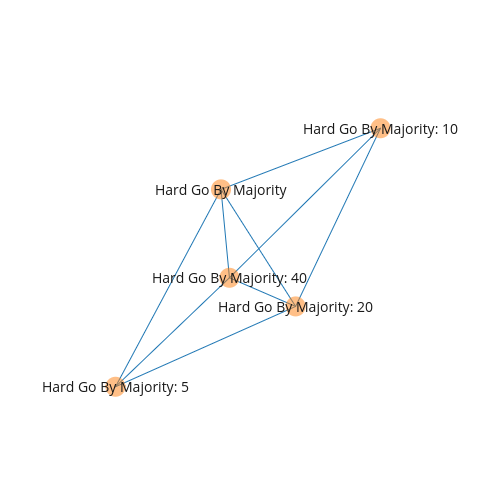
\includegraphics[width = 0.3\textwidth]{../img/neighbourhoods/60.png}\label{fig:nbh_hard_gbm}}
\subfloat[]{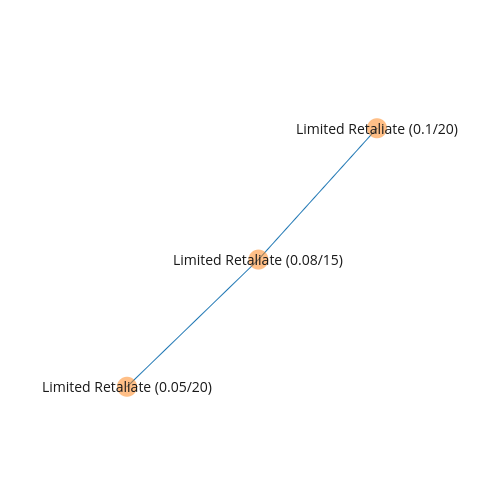
\includegraphics[width = 0.3\textwidth]{../img/neighbourhoods/7.png}}
\subfloat[]{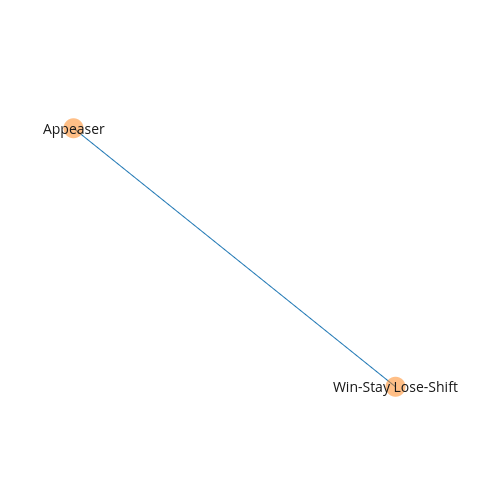
\includegraphics[width = 0.3\textwidth]{../img/neighbourhoods/74.png}} \\
\phantomcaption
\end{figure}
\begin{figure}[htbp!]
\ContinuedFloat
\subfloat[]{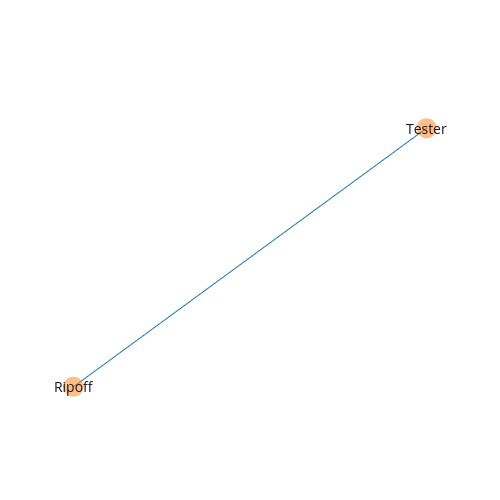
\includegraphics[width = 0.3\textwidth]{../img/neighbourhoods/78.png}}
\subfloat[]{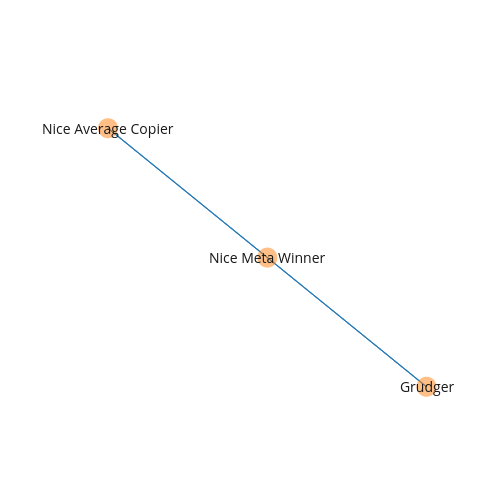
\includegraphics[width = 0.3\textwidth]{../img/neighbourhoods/84.png}}\\

\caption{All the disjoint neighbourhoods from Figure \ref{fig:overall_neighbourhoods}}
\label{fig:sep_neighbourhoods}
\end{figure}
